\subsection{Real-fault operating curve}
\label{sec:operating-curve}
On the Intel Berkeley Lab deployment, the composed system detects real battery-depletion faults at a high rate while keeping healthy false alarms low, and the operator can trade the two by moving a single mean-threshold operating point. Table~\ref{tab:operating} reports the pooled sweep over motes ($N_\mathrm{healthy} \approx 1.52$M healthy samples, $N_\mathrm{fault} \approx 0.39$M fault samples; \texttt{i7\_intel\_lab\_operating\_points.csv}). At a mean threshold of $8.0$ the system reaches a $7.4\%$ healthy false-positive rate at $90.1\%$ real-fault detection; lowering the threshold to $3.0$ raises detection to $92.6\%$ at the cost of a $22.1\%$ false-positive rate. The detection rate is remarkably flat across the sweep (from $0.926$ down to $0.901$), so the operating point is chosen almost entirely by the tolerable false-alarm budget.

\begin{table}[t]
    \centering
    \caption{Real battery-depletion fault detection on the Intel Berkeley Lab deployment, online adaptive detector, pooled over motes. Source: \texttt{i7\_intel\_lab\_operating\_points.csv} ($N_\mathrm{healthy}=1\,518\,828$, $N_\mathrm{fault}=387\,671$).}
    \label{tab:operating}
    \begin{tabular}{rcc}
        \toprule
        Mean threshold & Healthy FP rate & Real-fault detection \\
        \midrule
        3.0 & 0.221 & 0.926 \\
        4.0 & 0.165 & 0.916 \\
        5.0 & 0.129 & 0.910 \\
        6.0 & 0.104 & 0.906 \\
        8.0 & 0.074 & 0.901 \\
        \bottomrule
    \end{tabular}
\end{table}

\begin{figure}[t]
    \centering
    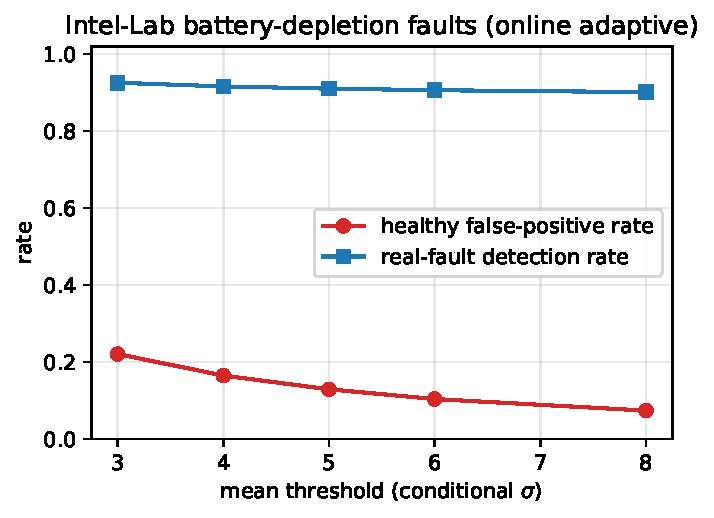
\includegraphics[width=0.8\linewidth]{figures/fig_operating_curve.pdf}
    \caption{Operating curve on the Intel Berkeley Lab battery-depletion faults (online adaptive detector, pooled over motes). Raising the mean threshold trades a lower healthy false-positive rate against a marginal drop in real-fault detection. Source: \texttt{i7\_intel\_lab\_operating\_points.csv}.}
    \label{fig:operating}
\end{figure}

Online adaptation is mandatory on this stream, not a convenience. A static model fit on a short prefix of the same diurnal signal false-alarms at a rate of $0.97$: the daily temperature and humidity cycle alone is enough to push a fixed model permanently out of distribution. The adaptive detector tracks the diurnal baseline and reserves its alarms for the battery-depletion excursions.

The types assigned to the detected real faults are dominated by freezing, as a stuck-at-degraded-value failure should be. Table~\ref{tab:realtypes} reports the type distribution over detected real-fault samples (\texttt{i7\_intel\_lab\_fault\_types.csv}): $93.2\%$ are typed freezing, $5.1\%$ drift, $1.7\%$ bias, and $0.06\%$ accuracy loss. The freezing label corresponds to the physical reality of a transmitter pinned at a corrupted reading as its battery fails, so the typing layer converts the detector's alarm into the maintenance-relevant diagnosis ``replace the mote'' rather than ``investigate the process.''

\begin{table}[t]
    \centering
    \caption{Fault types assigned to detected real faults on the Intel Berkeley Lab deployment. Source: \texttt{i7\_intel\_lab\_fault\_types.csv}.}
    \label{tab:realtypes}
    \begin{tabular}{lrr}
        \toprule
        Assigned type & Count & Fraction \\
        \midrule
        freezing      & 578\,721 & 0.932 \\
        drift         & 31\,727  & 0.051 \\
        bias          & 10\,395  & 0.017 \\
        accuracy loss & 343      & 0.001 \\
        \bottomrule
    \end{tabular}
\end{table}

The residual healthy false positives are themselves informative. Approximately $93\%$ of healthy false positives are typed as drift, arising from the healthy diurnal ramps that the two-signal conditional model (temperature given humidity, and vice versa) cannot fully cancel. This is an honest limitation tied directly to the correlation-dependence we characterize in Section~\ref{sec:regime}: with only two correlated signals available, slow shared ramps leak into the residual; a deployment with more correlated signals would suppress them further.

\subsection{Per-type recall and the bias--coupling relationship}
\label{sec:per-type}
On the scaled controlled injections, the four types are recovered at sharply different rates. Table~\ref{tab:pertype} reports per-type recall with Wilson 95\% confidence intervals over $N=85$ trials per type (\texttt{i7\_scaled\_per\_type.csv}). Freezing is recovered perfectly ($1.000$, CI $0.957$--$1.000$) and drift well ($0.741$), while accuracy loss ($0.659$) and especially bias ($0.518$) are lower. Cross-talk precision on normal peer signals is high: of the signals labelled by typing, the normal-peer label is correct with precision $\approx 0.91$ (\texttt{i7\_scaled\_normal\_precision.csv}), so coupled peers are rarely misattributed a fault.

\begin{table}[t]
    \centering
    \caption{Per-type recall on scaled controlled injections, $N=85$ trials per type, Wilson 95\% CI. Source: \texttt{i7\_scaled\_per\_type.csv}.}
    \label{tab:pertype}
    \begin{tabular}{lccc}
        \toprule
        Fault type & Recall & 95\% CI & $N$ \\
        \midrule
        freezing      & 1.000 & [0.957, 1.000] & 85 \\
        drift         & 0.741 & [0.639, 0.822] & 85 \\
        accuracy loss & 0.659 & [0.553, 0.751] & 85 \\
        bias          & 0.518 & [0.413, 0.621] & 85 \\
        \bottomrule
    \end{tabular}
\end{table}

The aggregate bias recall of $0.518$ is not an unexplained weakness; it is the mean of two distinct regimes. Table~\ref{tab:biascoupling} reports bias recall per target channel against that channel's conditional standard deviation $\sigma$ (\texttt{i7\_scaled\_bias\_by\_channel.csv}). Bias recall is monotone in $\sigma$: on strongly coupled channels (small conditional $\sigma$, because peers explain most of the variance) the recall is near-perfect ($0.941$ at $\sigma=0.216$, $1.000$ at $\sigma=0.480$), whereas on weakly coupled channels (large conditional $\sigma$) it collapses ($0.353$, $0.235$, down to $0.059$ at $\sigma=1.471$). This is the key finding of the characterization: the interpretable conditional model \emph{absorbs} a constant offset on a strongly coupled signal, because the conditional mean tracks the offset through the peers, while it \emph{isolates} the same offset on a weakly coupled signal. The aggregate $0.52$ is thus the average of an ``isolable'' regime and an ``absorbed'' regime, not a uniformly mediocre detector.

\begin{table}[t]
    \centering
    \caption{Bias recall is monotone in conditional standard deviation $\sigma$: offsets are absorbed on strongly coupled (small-$\sigma$) channels and isolated on weakly coupled (large-$\sigma$) channels. $N=17$ per channel, Wilson 95\% CI. Source: \texttt{i7\_scaled\_bias\_by\_channel.csv}.}
    \label{tab:biascoupling}
    \begin{tabular}{lcccc}
        \toprule
        Channel & Conditional $\sigma$ & Bias recall & 95\% CI & $N$ \\
        \midrule
        bed2 & 0.216 & 0.941 & [0.73, 0.99]  & 17 \\
        bed1 & 0.480 & 1.000 & [0.816, 1.00] & 17 \\
        bso1 & 1.439 & 0.353 & [0.173, 0.587] & 17 \\
        bfo2 & 1.443 & 0.235 & [0.096, 0.473] & 17 \\
        cso1 & 1.471 & 0.059 & [0.01, 0.27]  & 17 \\
        \bottomrule
    \end{tabular}
\end{table}

\begin{figure}[t]
    \centering
    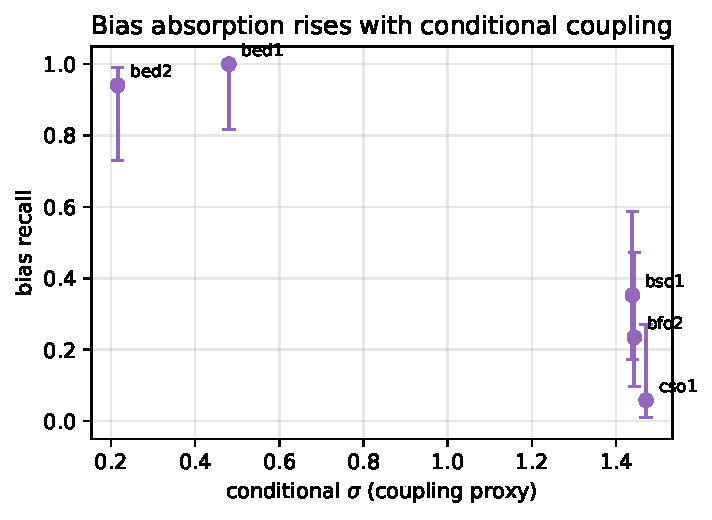
\includegraphics[width=0.8\linewidth]{figures/fig_bias_vs_sigma.pdf}
    \caption{Bias recall is monotone in conditional $\sigma$: a constant offset is isolated on weakly coupled (small-$\sigma$) channels and absorbed by the conditional mean on strongly coupled (large-$\sigma$) channels. Error bars are Wilson 95\% intervals. Source: \texttt{i7\_scaled\_bias\_by\_channel.csv}.}
    \label{fig:biascoupling}
\end{figure}

\subsection{Real bias and the detection floor}
\label{sec:lbnl}
The bias--coupling relationship above predicts that a constant offset is isolable only when it is large relative to the conditional scale of the signal it perturbs. We confirm this on a real labelled-fault dataset: the LBNL building-FDD MZVAV-1 set~\citep{LBNL_FDD2019,Granderson2023}, in which a constant offset of $\pm 1$, $\pm 2$, or $\pm 4\,^\circ$C is imposed on the outdoor-air-temperature sensor of a simulated multi-zone air-handling unit, with a per-timestamp fault label. We run the online adaptive detector over the four coupled AHU air temperatures (supply, outdoor, mixed, return), holding out the fault label, and measure typing on the biased outdoor-air-temperature signal (\texttt{i7\_lbnl\_bias.csv}).

The decisive quantity is the magnitude of the imposed bias in conditional-standard-deviation units. The outdoor-air-temperature conditional standard deviation on healthy data is $3.81\,^\circ$F, so the imposed offsets ($1.8$, $3.6$, $7.2\,^\circ$F) correspond to only $0.47$, $0.94$, and $1.89\,\sigma$ respectively---every one of them below the $3\sigma$ isolation threshold. The detector therefore correctly declines to flag them: detection of the biased signal is $0.27$--$0.33$ across the threshold sweep, and forcing detection upward by lowering the mean threshold to $2\sigma$ drives the healthy false-positive rate to $0.74$ (Table~\ref{tab:lbnl}). This is not a failure but a quantified \emph{detection floor}: a threshold-based typing layer isolates a bias only once it exceeds a few conditional standard deviations, by construction, and alarming below that floor would flood the operator with false positives. The result triangulates with the controlled study, whose injections at $4\sigma$ (above the floor) were isolable, and with the bias--coupling relationship: real sensor biases that are small relative to a signal's conditional scale are, and should be, below the alarm floor.

\begin{table}[t]
    \centering
    \caption{Real outdoor-air-temperature bias on LBNL MZVAV-1 (online adaptive detector). The imposed offsets are $0.47$--$1.89\,\sigma$, below the $3\sigma$ floor, so detection is low and cannot be raised without an unacceptable false-positive rate. Source: \texttt{i7\_lbnl\_bias.csv}.}
    \label{tab:lbnl}
    \begin{tabular}{rccc}
        \toprule
        Mean threshold & Healthy FP rate & Bias detection & Typed as bias \\
        \midrule
        2.0 & 0.743 & 0.332 & 0.034 \\
        3.0 & 0.686 & 0.302 & 0.018 \\
        4.0 & 0.657 & 0.280 & 0.009 \\
        5.0 & 0.634 & 0.269 & 0.006 \\
        \bottomrule
    \end{tabular}
\end{table}

\subsection{Freezing is type attribution, not detection capability}
\label{sec:freeze}
We initially expected freezing to be a detection blind spot of the base detector, on the reasoning that a signal stuck at a value within its normal range would not trigger a conditional-CDF alarm. This claim is refuted by our own validation. Table~\ref{tab:freeze} reports, per channel, the base CDF detection rate, the dedicated freeze-test detection rate, their median detection delays, and the fraction of trials in which the freeze test fired earlier (\texttt{i7\_freeze\_latency.csv}). The base CDF detector catches \emph{every} injected freeze on \emph{every} channel ($\texttt{cdf\_detect\_rate}=1.0$, $\texttt{frac\_cdf\_never}=0.00$ throughout), because the conditional expectation keeps moving while the frozen signal does not, driving the residual out of bounds. Moreover, the CDF detector is usually \emph{faster}: its median delay ranges from $2$ to $28$ steps, and the freeze test---whose fixed $25$-step confirmation window sets its median delay at exactly $25$---fires earlier in only about half the trials, and only on the most isolated channel (bed2, $\texttt{frac\_freeze\_earlier}=0.529$); on the most coupled channels it never beats the CDF detector ($0.0$).

\begin{table}[t]
    \centering
    \caption{Freezing detection: the base CDF detector catches every injected freeze on every channel, usually faster than the fixed $25$-step freeze test. Source: \texttt{i7\_freeze\_latency.csv} ($N=17$ per channel).}
    \label{tab:freeze}
    \begin{tabular}{lccccc}
        \toprule
        Channel & Cond.\ $\sigma$ & CDF detect & CDF median delay & Freeze earlier & CDF never \\
        \midrule
        bed2 & 0.216 & 1.0 & 28 & 0.529 & 0.0 \\
        bed1 & 0.480 & 1.0 & 9  & 0.294 & 0.0 \\
        bso1 & 1.439 & 1.0 & 17 & 0.412 & 0.0 \\
        bfo2 & 1.443 & 1.0 & 3  & 0.000 & 0.0 \\
        cso1 & 1.471 & 1.0 & 2  & 0.000 & 0.0 \\
        \bottomrule
    \end{tabular}
\end{table}

The conclusion is that the freeze test adds type \emph{attribution}---distinguishing a stuck sensor from a genuine process excursion---rather than detection capability or speed. The theoretical blind spot, in which the conditional standard deviation collapses to zero and the residual cannot grow, is an edge case that does not arise in the real or injected data we examined. On the real deployment this attribution is exactly what types the battery-depletion faults as freezing (Section~\ref{sec:operating-curve}), turning a detection into a maintenance label.

\subsection{Regime robustness comes from suppression, not residual cancellation}
\label{sec:regime}
We also expected the conditional residual to cancel coordinated shifts---a fault arriving as a shared shift across correlated signals would, on this reasoning, leave the conditional residual unchanged and so produce no spurious type label, independent of the change-point suppression. This claim is also refuted: residual cancellation (mechanism~1) is strongly correlation-dependent, and the robustness of the composed system instead comes from graded change-point suppression (mechanism~2). Table~\ref{tab:regime} reports the false-label rate across correlation $\rho$, coordinated-shift magnitude, and suppression scale (\texttt{i7\_regime\_fp.csv}, $5$ seeds per cell). With suppression disabled ($\texttt{scale}=1$), a $\geq 6\sigma$ coordinated shift at low correlation ($\rho=0.1$) produces about $20\%$ false labels ($0.199$ at $6\sigma$, $0.201$ at $10\sigma$); the boundary recedes as $\rho$ increases and is gone by $\rho \geq 0.7$. By contrast, the default graded suppression ($\texttt{scale}=5$) drives the false-label rate to exactly $0.0$ in every $(\rho, \text{shift})$ cell, as does full suppression ($\texttt{scale}=\infty$).

\begin{table}[t]
    \centering
    \caption{False-label rate under coordinated shifts co-occurring with a change point, by correlation $\rho$, shift magnitude, and suppression scale (mean over $5$ seeds). Residual cancellation alone ($\texttt{scale}=1$) fails at low correlation; graded suppression ($\texttt{scale}=5$) yields $0.0$ everywhere. Source: \texttt{i7\_regime\_fp.csv}.}
    \label{tab:regime}
    \begin{tabular}{ccccc}
        \toprule
        $\rho$ & Shift ($\sigma$) & \texttt{scale}=1 & \texttt{scale}=5 & \texttt{scale}=$\infty$ \\
        \midrule
        0.1 & 3  & 0.000 & 0.000 & 0.000 \\
        0.1 & 6  & 0.199 & 0.000 & 0.000 \\
        0.1 & 10 & 0.201 & 0.000 & 0.000 \\
        0.3 & 3  & 0.000 & 0.000 & 0.000 \\
        0.3 & 6  & 0.021 & 0.000 & 0.000 \\
        0.3 & 10 & 0.198 & 0.000 & 0.000 \\
        0.5 & 3  & 0.000 & 0.000 & 0.000 \\
        0.5 & 6  & 0.000 & 0.000 & 0.000 \\
        0.5 & 10 & 0.112 & 0.000 & 0.000 \\
        0.7 & 3--10 & 0.000 & 0.000 & 0.000 \\
        0.9 & 3--10 & 0.000 & 0.000 & 0.000 \\
        \bottomrule
    \end{tabular}
\end{table}

The adapt-into-drift robustness of the composed system therefore rests on mechanism~2, the graded change-point suppression, and not on the conditional-residual cancellation we originally credited. This matters operationally: the suppression scale is the parameter the operator must set, and it has a measurable cost, quantified next.

\begin{figure}[t]
    \centering
    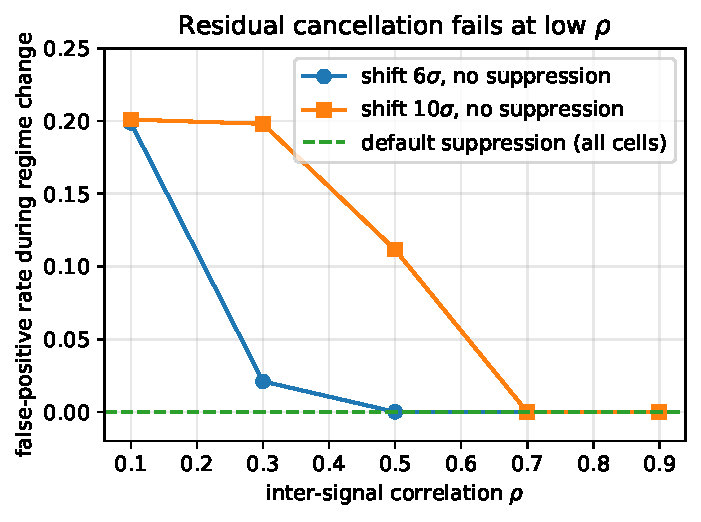
\includegraphics[width=0.8\linewidth]{figures/fig_regime_fp.pdf}
    \caption{Without change-point suppression, conditional-residual cancellation (mechanism~1) fails at low correlation: a large coordinated shift produces false fault labels until $\rho$ is high. The default graded suppression (mechanism~2) drives the rate to zero in every cell. Source: \texttt{i7\_regime\_fp.csv}.}
    \label{fig:regime}
\end{figure}

\subsection{The cost of suppression: dead-band and freeze-on-quiescent ablations}
\label{sec:ablation}
Suppression suppresses real faults too. Table~\ref{tab:deadband} reports the detection of a genuine drift that co-occurs with a change point, as a function of suppression scale (\texttt{i7\_deadband.csv}, $5$ seeds). With no suppression ($\texttt{scale}=1$) the drift is detected once it reaches $5.2\sigma$; at the default $\texttt{scale}=5$ detection is delayed until $17.6\sigma$; at $\texttt{scale}=\infty$ the drift is never detected. The default suppression thus opens a masking dead-band of roughly $[3\sigma, 15\sigma]$ for faults that happen to coincide with a change point---the measured price of the robustness reported in Section~\ref{sec:regime}.

\begin{table}[t]
    \centering
    \caption{Co-occurring-fault dead-band: detection magnitude of a drift co-occurring with a change point, by suppression scale ($5$ seeds). Source: \texttt{i7\_deadband.csv}.}
    \label{tab:deadband}
    \begin{tabular}{lccc}
        \toprule
        Suppression scale & Detected & Median delay & Magnitude at detection ($\sigma$) \\
        \midrule
        1.0      & yes & 26 & 5.2  \\
        5.0      & yes & 88 & 17.6 \\
        $\infty$ & no  & -- & --   \\
        \bottomrule
    \end{tabular}
\end{table}

\begin{figure}[t]
    \centering
    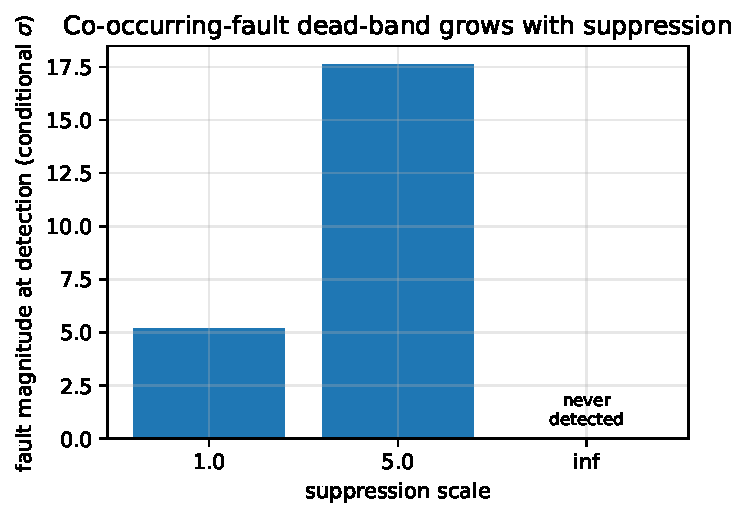
\includegraphics[width=0.7\linewidth]{figures/fig_deadband.pdf}
    \caption{The co-occurring-fault dead-band: a drift co-occurring with a change point must grow from $5.2\sigma$ (no suppression) to $17.6\sigma$ (default suppression) before detection, and is never detected under full suppression. Source: \texttt{i7\_deadband.csv}.}
    \label{fig:deadband}
\end{figure}

The freeze test similarly requires calibration on steady-state signals. Table~\ref{tab:quiescent} reports the false freeze-label rate on a genuinely live but very quiet signal (noise at $0.5\%$ of the marginal standard deviation) under three freeze-constant settings (\texttt{i7\_freeze\_quiescent.csv}, $5$ seeds). With the default constants, such a signal is falsely labelled frozen $72\%$ of the time; the loose constants make it worse ($\approx 88\%$); the strict constants ($\texttt{freeze\_eps}=10^{-4}$, $\texttt{freeze\_var\_ratio}=5\times10^{-3}$, $\texttt{freeze\_abs\_scale}=5$) eliminate the false label entirely ($0.0$). We therefore recommend the strict constants, or per-signal calibration, for deployments containing steady-state signals.

\begin{table}[t]
    \centering
    \caption{Freeze-on-quiescent ablation: false freeze-label rate on a live but quiet signal (noise $0.5\%$ of marginal std), by freeze-constant setting ($5$ seeds). Source: \texttt{i7\_freeze\_quiescent.csv}.}
    \label{tab:quiescent}
    \begin{tabular}{lccc}
        \toprule
        Freeze constants & \texttt{freeze\_eps} & \texttt{freeze\_var\_ratio} / \texttt{freeze\_abs\_scale} & False freeze rate \\
        \midrule
        default & $1\times10^{-3}$ & $1\times10^{-2}$ / $20$ & 0.717 \\
        loose   & $5\times10^{-3}$ & $5\times10^{-2}$ / $50$ & 0.887 \\
        strict  & $1\times10^{-4}$ & $5\times10^{-3}$ / $5$  & 0.000 \\
        \bottomrule
    \end{tabular}
\end{table}

\subsection{Detection baseline}
\label{sec:baseline}
Because the typing layer is only as useful as the detector beneath it, we confirm that the base detector is competitive with a published streaming alternative. Table~\ref{tab:baseline} compares it against the streaming autoencoder detector of \citet{Reunanen2020}---a one-pass, no-window outlier detector---under identical online point-wise evaluation on the SKAB multivariate benchmark ($37\,222$ points, $35.4\%$ anomalous; \texttt{i5\_reunanen\_skab.csv}). The base conditional-Gaussian detector outperforms the baseline on both threshold-free ROC AUC ($0.562$ vs $0.499$) and best-case F1 ($0.452$ vs $0.414$). Absolute values are modest because SKAB's anomalies are collective events that point-wise scoring penalises for any memory-less one-pass detector; the comparison is a relative positioning of the detector our typing layer extends, not a state-of-the-art detection claim.

\begin{table}[t]
    \centering
    \caption{Detection head-to-head on SKAB, identical online point-wise evaluation. Source: \texttt{i5\_reunanen\_skab.csv}.}
    \label{tab:baseline}
    \begin{tabular}{lcc}
        \toprule
        Detector & ROC AUC & Best F1 \\
        \midrule
        Base (conditional Gaussian) & \textbf{0.562} & \textbf{0.452} \\
        \citet{Reunanen2020} (streaming autoencoder) & 0.499 & 0.414 \\
        \bottomrule
    \end{tabular}
\end{table}

\subsection{Benchmark positioning on TSB-AD}
\label{sec:tsbad}
The SKAB head-to-head fixes the detector's position against one streaming alternative; we now place it on a large, public, multi-domain benchmark. We evaluate on the univariate split of TSB-AD \citep{Liu2024TSBAD} (350 evaluation series spanning 23 source domains), under the strict one-pass \emph{predict-then-learn} regime: every point is scored before the model is allowed to learn from it, so no future information leaks into any score. Hyperparameters for the base detector and the \citet{Reunanen2020} baseline are tuned on the official disjoint tuning split by Bayesian optimisation with an identical budget; the z-score and random detectors are the standard reference floors. We report VUS-PR, the metric the TSB-AD authors identify as the most reliable for ranking detectors (\texttt{tsb\_ad\_fullrun.csv}).

Table~\ref{tab:tsbad} shows the base detector leads on mean VUS-PR ($0.335$ vs $0.271$ for the z-score, $0.164$ for \citet{Reunanen2020}, and $0.092$ for the random floor). The result is not driven by a few easy series: in paired per-series comparison the detector beats the z-score on $83\%$ of the 350 series, \citet{Reunanen2020} on $87\%$, and the random floor on $89\%$, and it is the single best method on $17$ of the $23$ source domains. The mean exceeds the median ($0.174$) because a minority of well-separated domains (e.g.\ Exathlon $0.80$, NEK $0.63$, YAHOO $0.59$) score highly while a long tail of hard point-anomaly domains (notably UCR, where every method scores below $0.03$) pulls the centre down. The z-score edges the detector on a handful of domains dominated by sharp, isolated spikes (MITDB, SMAP, Stock, TAO), where a memory-less point statistic is hard to beat; these are exactly the regimes least relevant to the slow sensor faults the typing layer targets. The headline, then, is that a constant-memory, one-pass detector with online adaptation is competitive with---and on average ahead of---a tuned streaming baseline across a broad public benchmark, which is the foundation the typing layer requires.

\begin{table}[t]
    \centering
    \caption{TSB-AD univariate split (350 series), strict one-pass predict-then-learn, VUS-PR. ``AID win'' is the fraction of series on which the base detector scores higher than the row method. Source: \texttt{tsb\_ad\_fullrun.csv}.}
    \label{tab:tsbad}
    \begin{tabular}{lccc}
        \toprule
        Method & Mean VUS-PR (95\% CI) & Median & AID win \\
        \midrule
        Base detector (AID) & \textbf{0.335} [0.299, 0.371] & \textbf{0.174} & --- \\
        z-score & 0.271 [0.240, 0.302] & 0.148 & 83\% \\
        \citet{Reunanen2020} & 0.164 [0.139, 0.188] & 0.069 & 87\% \\
        Random & 0.092 [0.074, 0.109] & 0.039 & 89\% \\
        \bottomrule
    \end{tabular}
\end{table}

\begin{figure}[t]
    \centering
    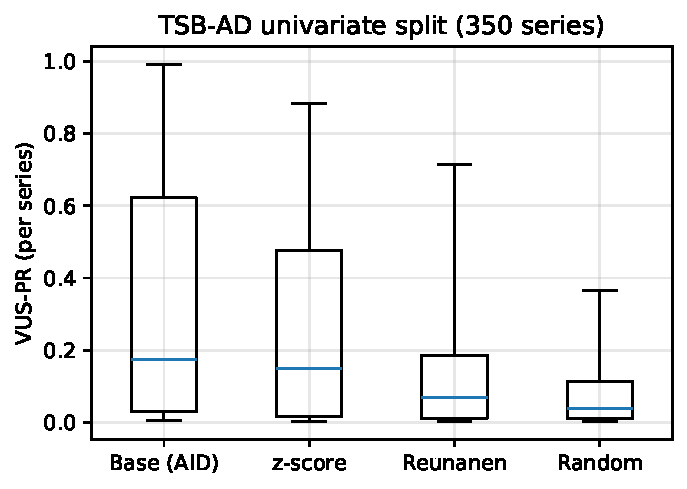
\includegraphics[width=0.7\linewidth]{figures/fig_tsbad_vuspr.pdf}
    \caption{Per-series VUS-PR distribution on the TSB-AD univariate split (350 series). Boxes span the interquartile range, whiskers the $5$th--$95$th percentiles; the base detector dominates both the median and the upper tail. Source: \texttt{tsb\_ad\_fullrun.csv}.}
    \label{fig:tsbad}
\end{figure}
